\subsection{Architecture}
\label{sec:archi}
\begin{figure}[h]
\begin{center}
\epsfig{file=archi.eps,width=\columnwidth}
\caption{PredicTV System Architecture}
\shrink
\label{fig:archi}
\end{center}
\end{figure}

The PredicTV system can be basically into four parts, 
showed in Figure \ref{fig:archi}. 
Communication module receives users' channel switching requests,
transfers them to Recommendation module, and outputs
recommendations to the user. Database module stores all the program
models and dynamically changing user viewing models. We next focus on
the other key components: information extraction module and
recommendation module.

The Information Extraction module has two tasks. One is to crawl HTML pages  
about TV programs from the internet, another is to extract 
important attribute-value pairs from the pages. 
We use Baidu and Google for the first task. 
%For a program
%that we want to collect its information, we form an URL based on Baidu
%and Google's rules. Then we send HTTP requests to both these two sites
%and get replies. Baidu and Google will reply the URLs of websites most fit
%the key word we provide, so we send HTTP requests again and get HTML files
%we need. Though Baidu and Google help us to search the websites most
%related to our key words, there will still be some noise in the HTML files,
%so we define some patterns to match information we need.

Recommendation module is the core of our system. It uses users' viewing
behaviour information as the
input of its analysis process then replies recommendation results to users
via Communication module. Since in mainland China, we don't have standard
and detailed TV program information available, we have to obtain such
information ourself. That's why Information Extraction module is involved
in our system. It grabs HTML files from the internet, filters unnecessary
parts, then passes them to Recommedation module. 


